\documentclass[aspectratio=169]{beamer}              % only frames

% for themes, etc.
\mode<presentation>
\usetheme{Madrid} 
\usecolortheme{crane}

%\usepackage{times}  % fonts are up to you
% The usual suspects
\usepackage{multirow, booktabs, dcolumn, color, graphicx} % Tables\usepackage{graphicx}
\usepackage{amsmath,amssymb,amsthm}
% Strikethrough text
\usepackage{soul}
% Adjust box to fit tabulars
\usepackage{adjustbox}
% Embed video
\usepackage{media9}
% For notes
\usepackage{pgfpages}
\setbeameroption{hide notes} % Only slides
%\setbeameroption{show only notes} % Only notes
%\setbeameroption{show notes on second screen=right} % Both
% Use colors by name
\usepackage{xcolor}
% EMBEDDING VIDEO IS POSSIBLE WITH PDFPC USE PDF PC to present
\usepackage{multimedia}



% The table highlighting for hypothesis discussion.
\usepackage[beamer,customcolors]{hf-tikz}
\usetikzlibrary{calc}

% To use background images
\newenvironment{colorframe}[2][]{%
\setbeamercolor{background canvas}{bg=#1}
\begin{frame}\color{white}}
{\end{frame}}


% To set the hypothesis highlighting boxes red.
\tikzset{hl/.style={
    set fill color=red!80!black!40,
    set border color=red!80!black,
  },
}

% Set Graphics folder
\graphicspath{{./figures/}}


% these will be used later in the title page
\title{Cryptography}
\subtitle{Cryptography Basics}
\author{Irfan Kanat}
\institute[CBS]{{Department of Digitization}\\ Copenhagen Business School}
%\date{\today}



\begin{document}

% this prints title, author etc. info from above
\begin{frame}

	\titlepage


	\vfill
	{\tiny \centering This work is licensed under a \href{http://creativecommons.org/licenses/by/4.0/}{Creative Commons Attribution 4.0 International License}.}

\end{frame}

\note{In this presentation we focus on cryptography basics up to symmetric key cryptography.}


\begin{frame}
	\frametitle{Big Question}
    
    \begin{itemize}
    	\item Securing information
    	\item Past efforts
    	\item Symmetric Key Cryptography
    \end{itemize}

\end{frame}

\note{In this video we will learn how to secure information starting with historical efforts and ending with Symmetric Key Cryptography.}

\begin{frame}
\frametitle{Securing Information}

\begin{columns}
	\begin{column}{0.5\textwidth}

		Securing Things

		\begin{itemize}
			\item Restrict Access
			\item Prevent Alterations
		\end{itemize}

		Securing Information is interesting.
	
	\end{column}

	\begin{column}{0.5\textwidth}

		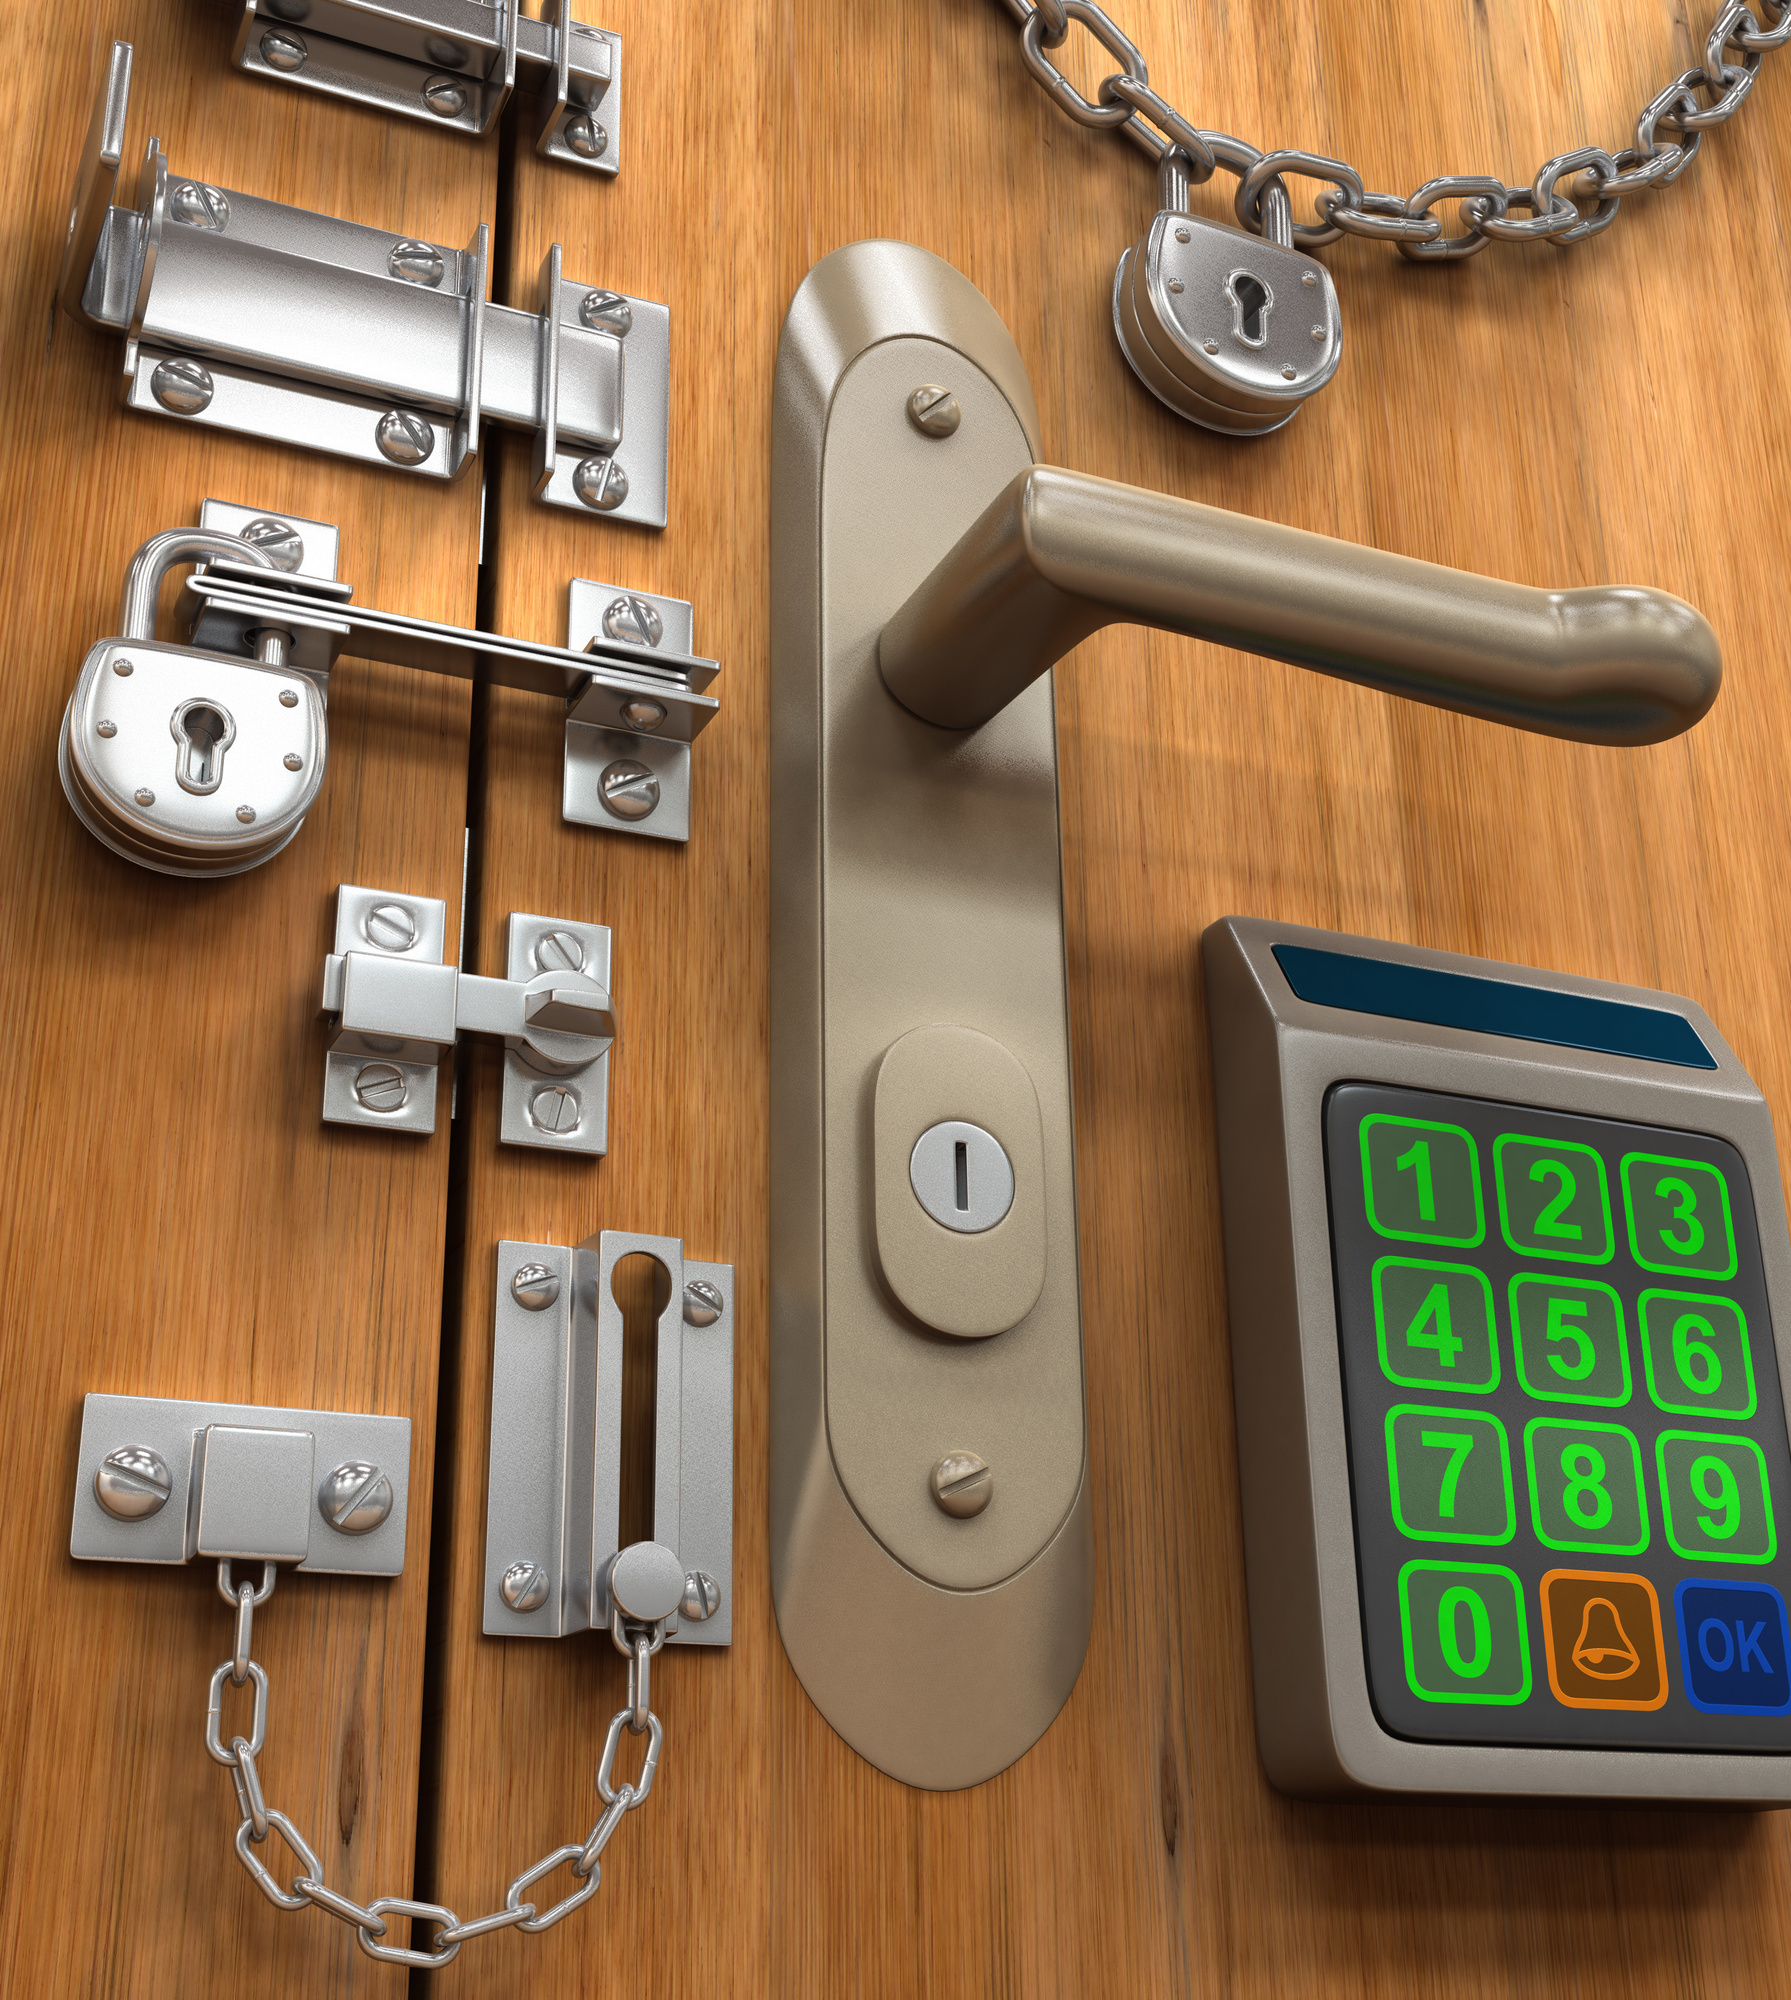
\includegraphics[width = \textwidth]{best-door-locks.jpeg}

	\end{column}

\end{columns}

\end{frame}

\note{
We all are engaged in securing things. We have doors to our houses with locks on. We have lockers with padlocks. We keep our belongings under our supervision when we are in situations where we can't control the environment.

What we do essentially is restricting access to our objects and preventing alteration of our objects. I would be very cross with you if you altered my lunch by eating it.

Information is interesting, because it is slightly different than physical objects. Unlike my lunch we can both consume the information and neither of us would be worse off. When you take information, you don't necessarily need to destroy the original. (This is the basis of a very weird argument about copyright violations being theft or not.)

Still there is value in keeping access and alteration of information in check. We employ clever technical solutions to limit access to and prevent alteration of information assets. There are whole businesses built around this idea: DRM, Cryptocurrencies, Blockchain technologies, and at the root of it all plain old encryption...

Today we will talk about encryption.}


\begin{frame}
	\frametitle{Ye Olde Encryption Schemes}
    
    \begin{columns}
		\begin{column}{0.5\textwidth}

		\only<1->{Substitution \vspace{1em}}


		\only<3->{Transposition \vspace{1em}}
		%\only<3-> One Time Pad \vspace{1em}
	
		\end{column}

		\begin{column}{0.5\textwidth}

		\only<1>{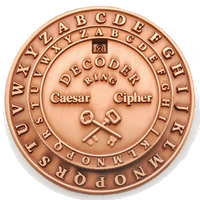
\includegraphics[width = \textwidth, height = .85\textheight, keepaspectratio]{figures/DecoderRing.png}}
		\only<2>{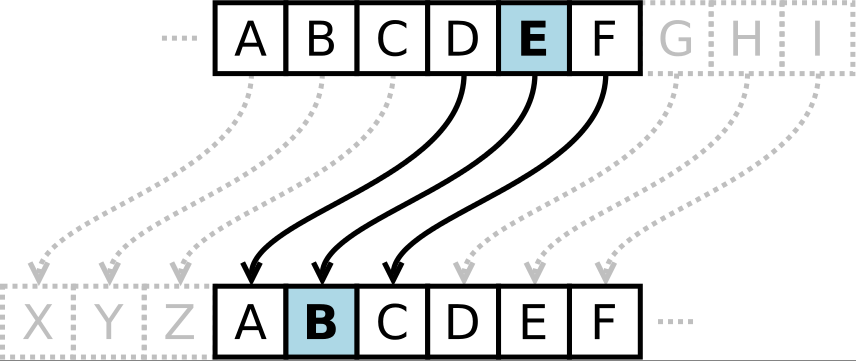
\includegraphics[width = \textwidth, height = .85\textheight, keepaspectratio]{figures/substitution.png} }
		\only<3>{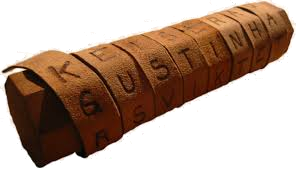
\includegraphics[width = \textwidth, height = .85\textheight, keepaspectratio]{figures/transposition0.png}}
		\only<4>{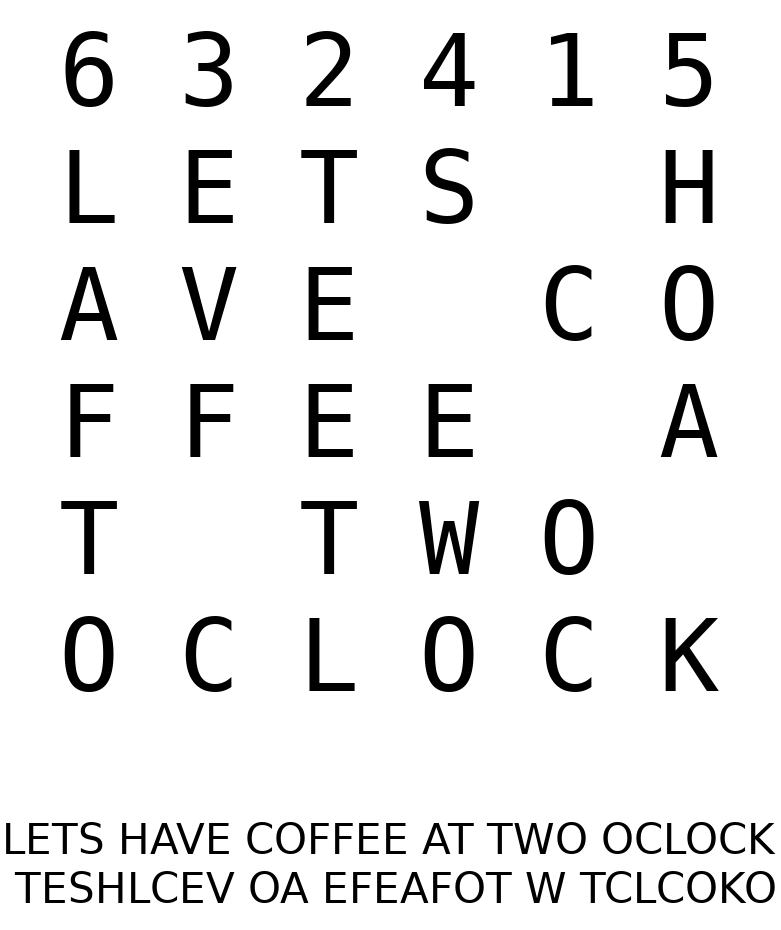
\includegraphics[width = \textwidth, height = .85\textheight, keepaspectratio]{figures/transposition.png} }
		%\only<3>{\includegraphics[width = \textwidth, height = .85\textheight, keepaspectratio]{figures/OneTimePad.jpeg}}

		\end{column}

	\end{columns}

\end{frame}

\note{Key take away, Caesar wasn't very cryptowise. There is only 26 possible keys afterall.

Simple substitution ala Caesar, and simple transposition of Spartan generals was good a thousand years ago.

The problem is these methods are open to brute force attacks or frequency analysis.

500 years ago, the most advanced crypto technology was to use polyalphabetic crypto. Having multiple substitution patterns and using a different one in round robin fashion... 

These days the only place you will find these methods is the puzzle books, and mystery novels.}

\begin{frame}
	\frametitle{Cryptography Basic Idea}

	\only<1>{
	Scrambling information in a reversible way \vspace{1em}

	Scrambled information looks like gibberish \vspace{1em}
	}

	\only<2>{
	\centering

	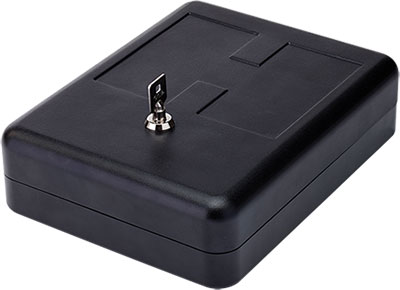
\includegraphics[width = \textwidth, height = .85\textheight, keepaspectratio]{figures/LockBox1.png} }
    
\end{frame}

\note{It is easy to imagine messages written on paper, but often it is harder to imagine what is happening to digital data in the computer.

A useful analogy is to imagine data being locked in a box. Locked with a key and unlocked with a copy of the same key.}


\begin{frame}
	\frametitle{Symmetric Key Cryptography}

	\centering

	{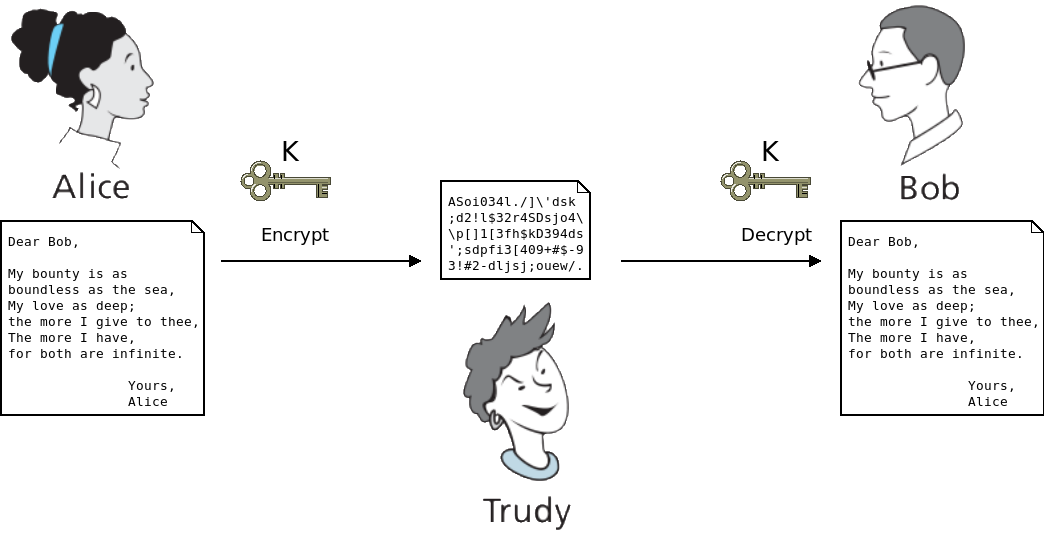
\includegraphics[width = \textwidth, height = .85\textheight, keepaspectratio]{figures/symmetricEncExample.png} }
	
\end{frame}

\note{If Alice and Bob have met before and shared a key,

Then they can encrypt and decrypt their messages without Trudy getting any wiser.

A single key both locks and unlocks the box and reveals the tender words of our lovers.
}

\begin{frame}
	\frametitle{Modern Cryptography}
    
    \centering
    {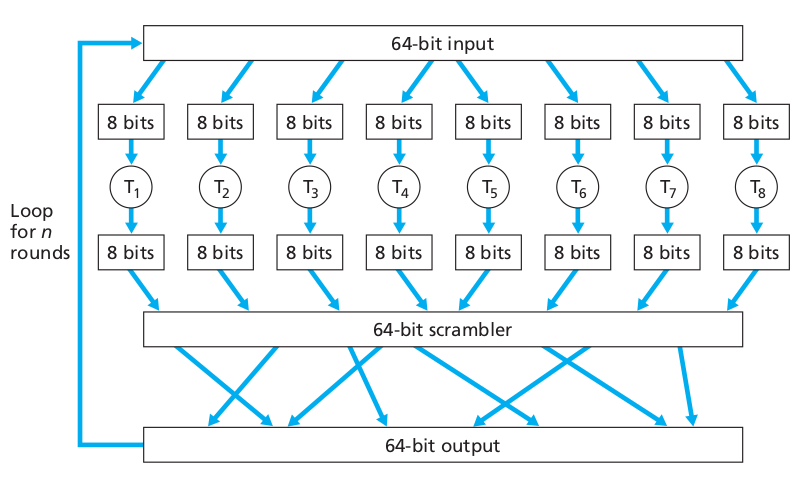
\includegraphics[width = \textwidth, height = .85\textheight, keepaspectratio]{figures/BlockCipher.png}}

\end{frame}

\note{
	With computers, bruteforcing immense numbers of trials became feasible. 

	This brought out a need for crypto systems with much larger solution spaces.

	Idea is computer can iterate over a crypto algorithm many times more complex than what people can.

	Above is a block cipher example like that of DES. Data is broken into blocks (of 8bits) and each block is processed by a different function to produce a different 8 bit block. The resulting blocks are scrambled and process repeated. After several iterations input bits will go through many different functions, resulting in end results that are vastly different from inputs.

	The DES algorithm (now defunct) used 56bit keys with 64bit blocks.

	AES uses larger block and key sizes (128, 256, 1024).

	If you were to brute force DES, it would require you to feed each of the possible keys ($2^{54} =  72057594000000000$) to the decryption algorithm. While this may appear difficult, breaking DES is trivial for modern computers.

	YET, the difficulty is exponential. If a computer can break 56bit keys in 1 seconds, it would take the same computer 149 trillion years to break a 128bit key and today we routinely use keys of sizes larger than 1024bits. (Best not talk about quantum computing and what it will do to our encryption yet).
}


{
\usebackgroundtemplate{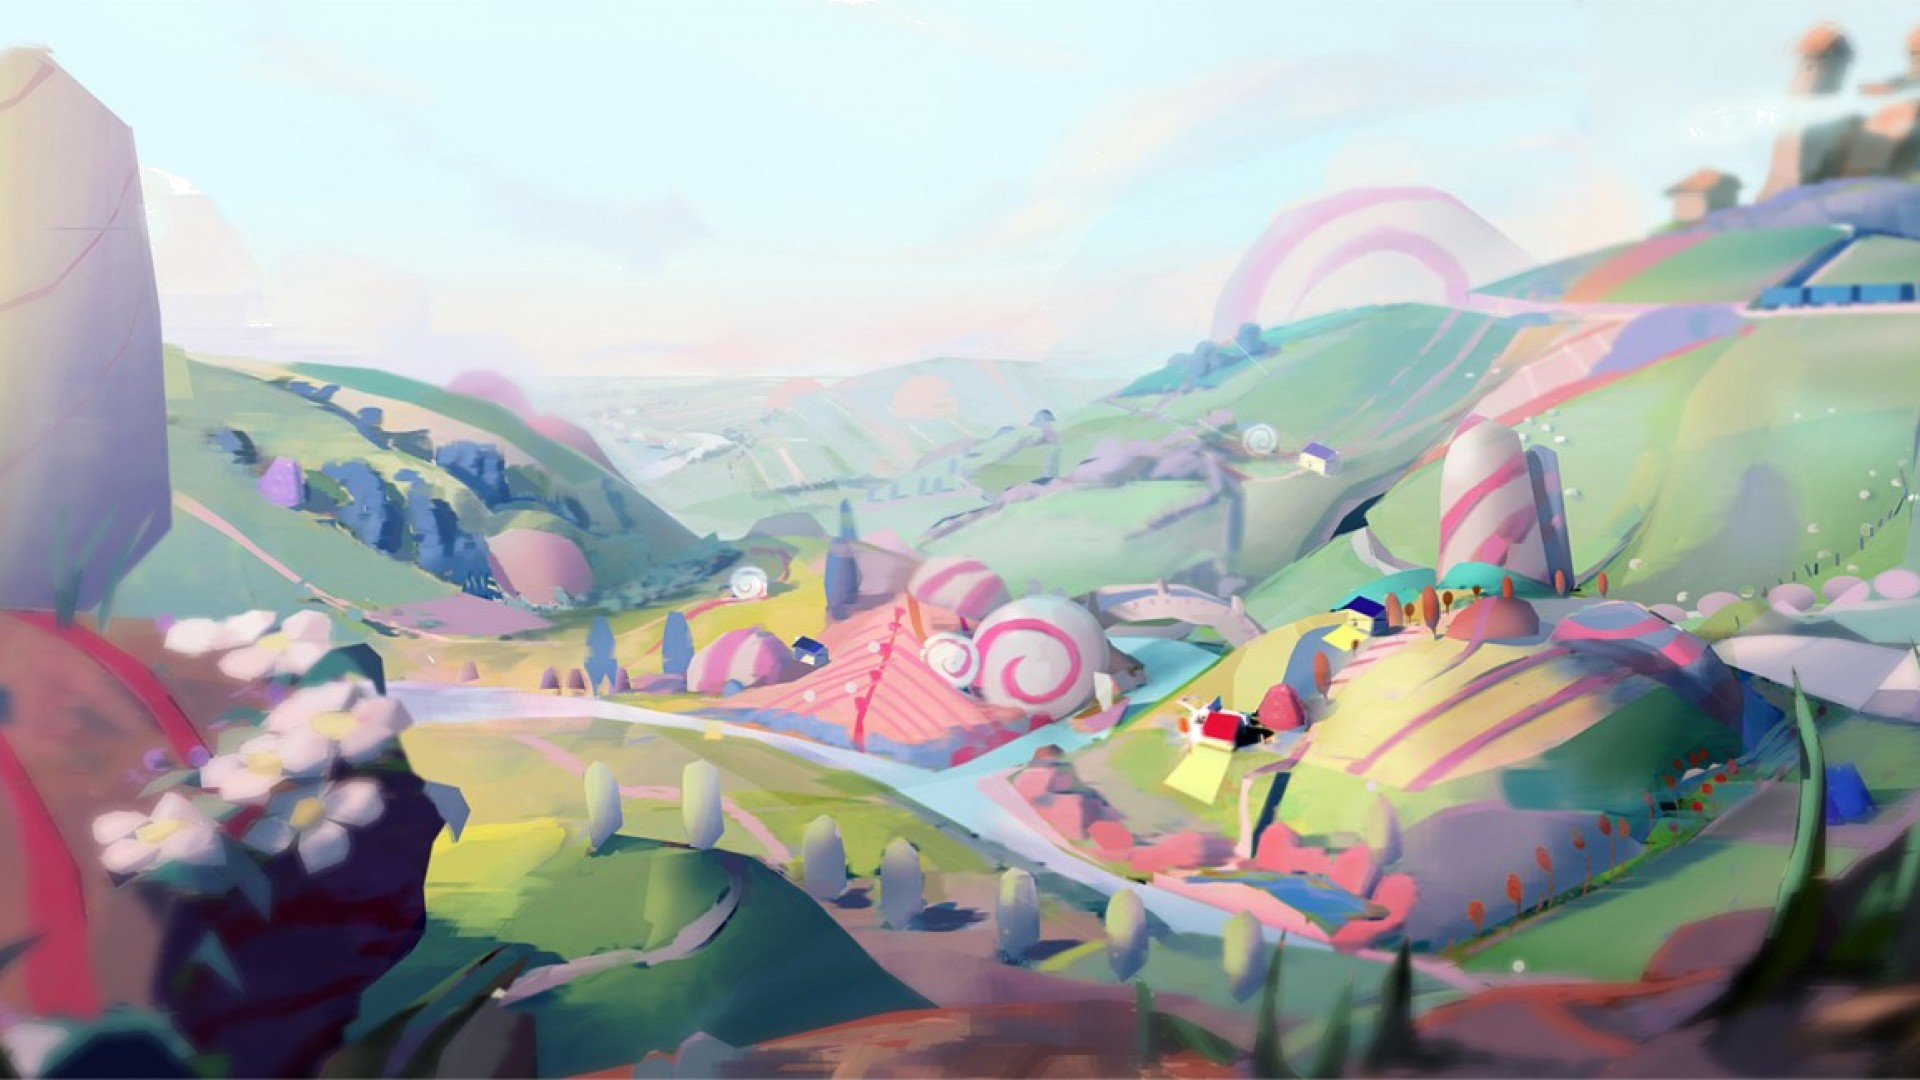
\includegraphics[width=\paperwidth,height=\paperheight]{demoland.png}}%
	\begin{frame}
	\frametitle{What Does Cryptography Look Like Really?}



	\end{frame}
}

\note{Goal here is to show the difference between cipher and clear text so the students can sort of get what is being done.

	You can say that you were touring Kronborg castle up near Helsingor and intercepted the message from the guards

	There is an encrypted cipher.txt file in the demo folder of this module.

		\# Show what is in the file:

		cat cipher.txt \# Or simply open with a text editor

	The file is gibberish, doesn't make sense

		\# Decrypt the file

 		openssl enc -des-ecb -d -in cipher.txt -K 1234 $>$ recovered.txt

 		\# Show what was recovered

 		cat recovered.txt

}

\begin{frame}
	\frametitle{Symmetric Key Cryptography}

	Light weight \vspace{1em}

	Straight forward \vspace{1em}
    
    Data at rest

\end{frame}

\note{Symmetric key cryptography is light weight compared to asymmetric key cyrptography. 

	Can be done faster.

	Easy to use without much hassle.

	Ideal for data at rest. That is data that is being stored for local use.

	Personally identifiable data (PID) of users are often encrypted this way.
}



\begin{frame}
	\frametitle{Recap}
    
    \begin{itemize}
    	\item Securing data
    	\item Past efforts
    	\item Symmetric Key Cryptography
    \end{itemize}

\end{frame}

\note{Internet is a jungle. It can be beautiful but you need to watch out for yourself. Things you do online have consequences IRL.}

\end{document}
